%*************************************************************************
%* Copyright © 2012 Vincent Prat & Simon Nicolas
%*
%* This document is free; you can redistribute it and/or modify
%* it under the terms of the GNU General Public License as published by
%* the Free Software Foundation; either version 3 of the License, or
%* (at your option) any later version.
%*
%* This document is distributed in the hope that it will be useful,
%* but WITHOUT ANY WARRANTY; without even the implied warranty of
%* MERCHANTABILITY or FITNESS FOR A PARTICULAR PURPOSE. See the
%* GNU General Public License for more details.
%*
%* You should have received a copy of the GNU General Public License along
%* with this document; if not, write to the Free Software Foundation, Inc.,
%* 51 Franklin Street, Fifth Floor, Boston, MA 02110-1301 USA.
%*************************************************************************

\documentclass[12pt]{article}
%\documentclass[12pt,twoside,french]{report}
%\documentclass[12pt]{proc}

\usepackage{fullpage}

\usepackage[frenchb]{babel}
\usepackage[utf8]{inputenc}
\usepackage{amsmath, graphicx}
\usepackage{hyperref}


\title{GM-Assistant, guide de l'utilisateur}
\author{
        Vincent Prat
            \and
        Simon Nicolas
}
\date{\today}


\begin{document}
\maketitle

%\begin{abstract}
%This is the paper's abstract \ldots
%\end{abstract}

\section{Introduction}
Une partie de jeux de rôle est une alchimie riche, et complexe. Les joueurs doivent être impliqués et investis, le maître de jeu (MJ) doit parfaitement maîtriser le système de règle, le scénario, se rappeler des évènements précédent, anticiper les évènements à venir, et improviser le présent en fonction des actions et choix des joueurs (PJ).
Si en pleine partie le MJ doit chercher des détails sur un PNJ, une précision sur un point de règle, des musiques d'ambiance ou des bruitages sur l'ordinateur, des images dans son classeur, ou autre, alors la partie ralenti, l'émulsion retombe, et les joueurs se dispersent.

La solution est GM-Assistant

GM-Assistant (pour Game-Master Assistant) est un logiciel d'assistant MJ. Son objectif est de simplifier la vie de MJ pendant les parties en mettant à sa disposition les informations et outils dont il peut avoir besoin pendant la partie.
Grâce à une interface claire, épurée, et efficace GMA met à la disposition du MJ tout ce dont il peut avoir besoin pendant une partie sans avoir besoin de chercher.

\section{Présentation des menus}\label{menu}
Dans la fenètre principale de GMA vous avez accès comme dans la plupat des logiciel à la barre des menus. Voici ce qu'ils contiennent:
\begin{itemize}
    \item \emph{Jeu :} permettant de gérer les fichiers de sauvegarde
    \begin{itemize}
        \item \emph{Nouveau :} Crée une nouvelle fiche scénario
        \item \emph{Recharger :} Restaure une fiche scénario telle qu'elle était lors de son dernier enregistrement
        \item \emph{Charger :} Charge une fiche scénario sctocker sur l'ordinateur
        \item \emph{Enregistrer :} Sauvegarde la fiche scénario en cours d'édition sur le disque
        \item \emph{Enregistrer sous :} Sauvegarde la fiche scénario en cours d'édition dans un nouveau fichier
        \item \emph{Récents :} Ouvre une listes des fiches scénario récemment ouvertes.
    \end{itemize} 
    \item \emph{Interface :} Ouvre la liste des arrangements de modules disponible. chaque interface propose un appariement différent de module à l'écran.
    \item \emph{?} Ouvre les informations générale sur le logiciel et ses licences.
\end{itemize}

\section{Présentation des modules}\label{modules}
GMA est organisé en module. Chaque module est indépendant et dédié à une fonctionnalité. Voici la liste des modules présent (en augmentation) au jour de \date{\today} :
\begin{itemize}
    \item \emph{Scénario :} l'arbre de scénario est un arbre "dépliable" qui permet d'afficher de manière ordonnée les différents évènements important du scénario. extensible à l'infini
    \item \emph{Notes :} éditeur de texte simpliste qui permet de prendre des notes pendant le scénario
    \item \emph{Personnages :} un tableau permettant d'afficher les protagoniste (PJ ou PNJ) avec leurs caractéristiques importantes
    \item \emph{Historique :} structurable en arbre aussi il a pour vocation à rappeler les évènements les plus marquant du scénario précédent
    \item \emph{Musique :} un lecteur de musique simple qui est pensé pour jouer (en boucle ou non) des musiques d'ambiance
    \item \emph{Personnages :} un tableau permettant d'afficher les protagoniste (PJ ou PNJ) avec leurs caractéristiques importantes
    \item \emph{Bruitages :} un lecteur de musique encore plus simple pensé pour déclencher au besoin des bruitage court
\end{itemize}
Tout ces modules sont rassemblées dans l'interface principale du logiciel :
\begin{figure}[h]
    \includegraphics[width=0.9\textwidth]{screen_scenar_exemple}
    \caption{Voici une capture de l'écran principale avec une partie en cours.
    ATTENTION il pourrait être mieux de faire une capture windows avec la barre des menus}
\end{figure}



\section{Les modules dans tous leurs états}\label{details}
Dans cette section nous rentrons dans le coeurs du sujet, nous allons découvrir en détail les fonctionnalités proposé par GMA, comment préparer sa partie, et comment utiliser GMA au mieux pendant la parties

\subsection{La notion d'item}\label{item}
Les items sont à la base du fonctionnement de GMA on les retrouve à de nombreux endroits dans le logiciel, il est donc approprié d'en expliquer le fonctionnement avant de détailler les modules.
Les modules qui utilisent les items sont : Scénario, Historique, Musique et Bruitage.

\begin{itemize}
    \item\emph{Clic droit dans le cadre vide du module} fait apparaitre la fenêtre "créer un item" (s'il n'y a aucun item)
    \item\emph{Clic droit sur un item} fait apparaitre le menu item contenant les 4 états disponible pour un item : \emph{Aucun}, \emph{En cours}, \emph{Echoué}, \emph{Réussi}, puis les 2 actions \emph{Ajouter} et \emph{Supprimer}
\end{itemize}
L'état d'un item permet de prendre note rapidement du succès ou de l'échec de certains points clefs du scénario, et d'en avoir une vision rapide.\\

\emph{Ajouter} nous permet d'accéder à la fenêtre de création d'item :
\begin{figure}[h]
    \includegraphics[width=0.5\textwidth]{screen_add_item}
    \caption{fenêtre d'ajout d'item}
\end{figure}
\begin{itemize}
    \item le cadre \emph{Contenu} reçoit la description de l'évènement/commentaire
    \item le cadre \emph{État} permet de fixer l'état de l'item
    \item le cade \emph{ype} permet de choisir si c'est un item "Basique", un "Son" ou une "Image", dans les 2 derniers cas le dernier cadre "Fichier" devient accessible pour aller chercher sur l'ordinateur le fichier requis
    \item Le bouton \emph{Ajouter} ajoute l'item à la suite et au même niveau que l'item sur lequel on a cliqué droit
    \item Le bouton \emph{Enfant} ajoute l'item à la suite et sous l'item sur lequel on a cliqué droit
    \item Le bouton \emph{Annuler} annule la création d'item en cours
\end{itemize}

Il est important de bien saisir la différence entre les 2 boutons \emph{Ajouter} et \emph{Enfant}
\emph{Nota Bene :} Les items sont déplaçable à la souris par \emph{cliquer déplacer}

\subsection{L'arbe de Scénario}\label{scenario}
L'arbre de scénario est dans la majorité des cas le cœur de GMA. En effet dedans il y a le plan détaillé et ordonné du scénario, de manière à ne jamais être perdu entre 2 scènes ni oublier un élément.
Voici un aperçu de ce que nous ce qu'il est possible de faire
\begin{figure}[h]
    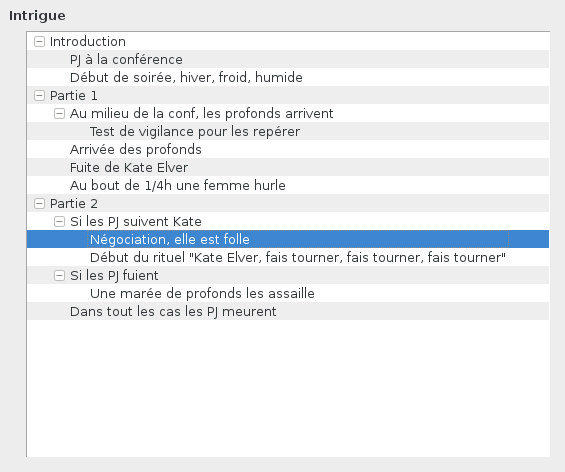
\includegraphics[width=0.6\textwidth]{scenario_type}
    \caption{Plan schématique d'un scénario}
\end{figure}
Donc comment faire ?
chaque ligne que vous voyez est un \emph{item}, donc il suffit de suivre la technique de création d'item pour ordonner son scénario.


\subsection{Prise de note rapide}
Le module de prise de note est un éditeur de texte ultra simpliste qui permet de noter à la volée toute information qui est utile à garder. Pour entrer du texte dedans il suffit de cliquer gauche quelque part dans le cadre texte et d'écrire.\\
\emph{Nota Bene :} ce module sera rapidement accessible lorsque la fonctionnalité de \emph{suivi de campagne} sera implémentée.

\subsubsection{Gestion des protagonistes}\label{personnage}
Le module \emph{personnages} est pensé pour accueillir la liste des protagonistes dont les caractéristiques numériques ont besoin d'être accessible rapidement. Que ce soit des PJ pour lesquels on a besoin des scores de Perception, vigilance, esquive passive, etc. ou directement des caractéristiques complètes des PNJ.
\\
Liste des actions possibles :
\begin{itemize}
    \item \emph{Clic droit $\rightarrow$ compétence} ajoute une compétence sur le bandeau horizontale
    \item \emph{Clic droit $\rightarrow$ personnage} ajoute un personnage sur le bandeau vertical 
\end{itemize}
Ensuite une fois qu'on a créé au moins un personnage et une compétence alors la case est éditable. Il faut maintenant cliquer gauche pour pour éditer la case voulue et y entrer la valeur.
\\\emph{Nota bene :} il est possible d'entrer du texte ou d'autre caractère comme le "\%"

Nous allons commencer par ajouter un personnage : Gros Bill, PJ joué par Pilou
\begin{figure}[h]
    \includegraphics[width=0.5\textwidth]{add_character}
    \caption{fenêtre d'ajout de personnage}
\end{figure}
FIXME Ensuite j'ai besoin de me rappeler en permanence de sa Force et de sa vigilance, je vais donc ajouter ces 2 caractéristiques.

\subsection{Musique d'ambiance}\label{musique}
Le module de musique d'ambiance est un lecteur de musique basique (loin des Winamp et autres Itunes) qui permet de jouer une musique (au format MP3)

Liste des actions possibles :
\begin{itemize}
    \item Actions des items cf (\ref{item})
    \item \emph{Clic gauche Lecture} joue le son sélectionné
    \item \emph{Clic gauche sur la case blanche "Boucle"} active le mode \emph{répétition} donc joue en boucle la musique de cours de lecture
    \item \emph{Clic gauche déplacer sur la barre d'avancement} permet de se déplacer dans le son
\end{itemize}
\emph{Nota Bene :} il est impossible de jouer 2 musiques en même temps.

\subsection{Les Bruitages}\label{bruitage}
Le module de bruitage est pensé pour accueillir une liste de son très court (au format MP3) limité en taille à 1Mo.

Liste des actions possibles :
\begin{itemize}
    \item Actions des items cf (\ref{item})
    \item \emph{Double clic gauche sur un item} joue le bruitage
\end{itemize}

Nota Bene : Il est tout fait possible de jouer un bruitage alors qu'une musique est en cours de lecture.

\section{Exemple de partie}\label{exemple}
Pour illustrer toute cette théorie il n'est rien de mieux d'un exemple de partie.
Voici donc notre scénario.
\begin{itemize}
    \item \emph{Titre du scénario :} La nuit tous les profonds sont gris
    \item \emph{Jeux de rôle :} L'appel de Cthulhu
    \item \emph{Année :} 1920
    \item \emph{Lieux :} Toulouse
    \item \emph{Nombre de joueurs : } 4
\end{itemize}

\emph{Scénario :}\\ 
Les PJ sont à l'inauguration du labo de pharma de la fac de médecine allée jules guesde, des profonds sortent de la garonne pour récupérer la dépouille d'un de leur chaman.
En même temps un des convives est un sorcier qui veut utiliser ce squelette pour en extraire de la puissance. Il profitera de la cohue des convives lors de l'assaut profond pour aller dans le labo, et commencer son rituel. La suite dépend des PJ. Si le rituel va au bout une onde de choc jette tout le monde à terre et les profonds fou de rage d'avoir perdu leur chaman définitivement assassinent tout le monde, sinon ils repartent tranquillement avec leur chaman (squelette)
\\
Aperçu de l'assistant créé pour :
\begin{figure}[h]
    \includegraphics[width=0.9\textwidth]{screen_scenar_exemple}
    \caption{La partie est prête}
\end{figure}

\section{Participer}\label{participer}
GMA c'est trop cool, vous n'envisagez plus de jouer sans et vous voulez participer au projets ?
Très bonne idée, nous sommes preneur de toute aide.
Le logiciel est placé sous license GPL3 et le projet est hébergé sur GitHub à cette adresse :
\href{http://vivicoder.github.com/GM-Assistant}{http://vivicoder.github.com/GM-Assistant}
%\url{http://vivicoder.github.com} ou un truc du genre 

\section{Conclusions}\label{conclusions}
GMA s'trop cool "T'AS VU !"
Home made, no inspiration expect 2 brilliant brain.

\section*{Nous contacter}
Pour les commentaires constructifs 2 autres adresses :
\begin{itemize}
    \item \href{mailto:dramac.nicolas@gmail.com}{dramac.nicolas@gmail.com}
    \item \href{mailto:vinceprat@free.fr}{vinceprat@free.fr}
\end{itemize}

\end{document}
